\section{Detailed Calculations}
\subsection{Calculation of the Power Spectrum}
In this Section we will perform the calculation for the observed power spectrum \todo{I need to add cdots for scalar products in this section...} $P^{\text{obs}}(\b \ell)$. For this, we assume an infinitely large field in order to perform our integration over $\mathbb{R}^2$. In reality, finite field effects would play a role here. We begin with the calculation of the correlation for the Fourier transformed shear:
\begin{align}
\la \gammaoh(\b \ell) \gammaoh {}^*(\b \ell')\ra = & \la\int\text{d}^2\b \theta\int\text{d}^2\b \theta'\,W(\b \theta)W(\b \theta')\gamma(\b \theta)\gamma^*(\b \theta')\exp(i\b \ell\b \theta-i\b \ell'\b \theta')\ra\nonumber\\
 = & \la\int\text{d}^2\b \theta\int\text{d}^2\b \theta'\,W(\b \theta)W(\b \theta')\exp(i\b \ell\b \theta-i\b \ell'\b \theta') \int \frac{\text{d}^2\b k}{(2\pi)^2}\int \frac{\text{d}^2\b k'}{(2\pi)^2}\, \hat{\gamma}(\b k)\hat{\gamma}^*(\b k')\exp(-i\b k\b \theta+i\b k'\b \theta')\ra \nonumber\\
= & \la \int \text{d}^2\b \theta \int \text{d}^2\b \theta' \int \frac{\text{d}^2\b k}{(2\pi)^2} \int \frac{\text{d}^2\b k'}{(2\pi)^2}\, P(\b k)(2\pi)^2 \delta(\b k-\b k') \exp[i(\b \ell\b \theta-\b \ell'\b \theta'-\b k\b \theta+\b k'\b \theta')]W(\b \theta)W(\b \theta')\ra \nonumber\\
  = & \la \int \frac{\text{d}^2\b k}{(2\pi)^2} \, P(\b k) \int \text{d}^2\b \theta\, W(\b \theta)\exp[i\b \theta(\b \ell-\b k)]\int \text{d}^2\b \theta'\, W(\b \theta') \exp[-i\b \theta(\b \ell'-\b k)] \ra \nonumber\\
  = & \la \int\frac{\text{d}^2 \b k}{(2\pi)^2} \, P(\b k)\widehat{W}(\b \ell-\b k)\widehat{W}^* (\b \ell'-\b k)\ra
\end{align}
It is important to keep in mind that the ensemble averages of the weight function are independent of the ensemble averages of the shear values, meaning $\la W(\b \theta)\gamma(\b \theta)\ra = \la W(\b \theta)\ra \la \gamma(\b \theta)\ra$. We can define $W(\b \theta)=1+w(\b\theta)$ with $\la w(\b \theta)\ra = 0$, which leads to the expession
\begin{align}
\la \gammaoh(\b \ell) \gammaoh {}^*(\b \ell')\ra = & \la \int\frac{\text{d}^2 \b k}{(2\pi)^2} \, P(\b k) \left[ (2\pi)^4\delta(\b \ell-\b k)\delta(\b \ell'-\b k)+(2\pi)^2\big( \hat{w}(\b \ell-\b k)\delta(\b \ell'-\b k) + \hat{w}^*(\b \ell'-\b k)\delta(\b \ell-\b k)\big)\right.\right. \nonumber\\
 & \qquad \left.\left. + \hat{w}(\b \ell-\b k)\hat{w}(\b \ell'-\b k) \right] \right. \bigg> \nonumber\\
 = & (2\pi)^2\delta(\b \ell-\b \ell')P(\b \ell) + \big[ \la \hat{w}(\b \ell-\b \ell')\ra P(\b \ell')+\la \hat{w}^*(\b \ell'-\b \ell)\ra P(\b \ell)\big] + \la \int \frac{\text{d}^2 \b k}{(2\pi)^2} \, \hat{w}(\b \ell-\b k)\hat{w}^*(\b \ell'-\b k)P(\b k)\ra \nonumber\\
\overset{(*)}{=} & (2\pi)^2\delta(\b \ell-\b \ell')P(\b \ell) + \la \int \frac{\text{d}^2 \b k}{(2\pi)^2}\, \hat{w}(\b \ell-\b k)\hat{w}^*(\b \ell'-\b k)P(\b k)\ra \, ,
\label{eq:pobs1}
\end{align}
where in $(*)$ we have used that the average $\la \hat{w}(\b \ell)\ra$ vanishes.
Up until now, we have not specified our weight-function $w$. So we now parametrize it as \begin{equation}
w(\b \theta) = \sum_{\b \alpha \in \mathbb{Z}^2} w_{\b \alpha} \Xi(\b \theta-L\b \alpha)\text{ , with the Box-Function } \Xi(\b \theta) = \begin{cases}
1 \qquad \b \theta\in \left[-\frac{L}{2},\frac{L}{2}\right]^2 \\
0 \qquad \text{else}
\end{cases}.
\end{equation}
Here, the $w_{\b \alpha}$ are random variables, drawn from the random distribution describing the survey depths. For the Fourier-Transform we compute: \begin{equation}
\hat{w}(\b \ell) = \sum_{\b \alpha \in \mathbb{Z}^2} w_{\b \alpha} \exp(-i \b \ell L\b \alpha) \widehat{\Xi}(\b \ell)\, ,
\end{equation}
where
\begin{equation}
\widehat{\Xi}(\b\ell) = \frac{4\sin\left(\frac{L\ell_1}{2}\right)\sin\left(\frac{L\ell_2}{2}\right)}{\ell_1\ell_2}\, ,
\end{equation}
is a 2-dimensional sinc function.
Assuming an uncorrelated weight-distribution $\left(\la w_{\b \alpha} w_{\b \beta}\ra = 0\text{ for }\b \alpha\neq\b \beta\right)$ and setting $\la w^2\ra \equiv \la w_{\b \alpha}^2\ra$ for each $\b \alpha$, we get
\begin{align}
\la \int \frac{\text{d}^2 \b k}{(2\pi)^2}\, \hat{w}(\b \ell-\b k)\hat{w}^*(\b \ell'-\b k)P(\b k)\ra = & \la \int \frac{\text{d}^2 \b k}{(2\pi)^2} \sum_{\b \alpha,\b \beta}w_{\b \alpha}w_{\b \beta} \exp[-i(\b \ell - \b k)L\b \alpha]\, \widehat{\Xi}(\b \ell - \b k) \exp[i(\b \ell' - \b k)L\b \beta]\, \widehat{\Xi}^*(\b \ell' - \b k)P(\b k)\ra \nonumber\\
 = & \int \frac{\text{d}^2 \b k}{(2\pi)^2} \sum_{\b \alpha} \la w^2\ra \exp[-i(\b \ell - \b k)L\b \alpha + i(\b \ell' - \b k) L\b \alpha]\, \widehat{\Xi}(\b \ell - \b k)\widehat{\Xi}^*(\b \ell' - \b k)P(\b k) \, .
\end{align}
Using this result, we can obtain the observed power spectrum \begin{equation}
P^{\rm{obs}}(\b\ell) = \frac{1}{(2\pi)^2}\int\d^2\ell' \la \gammaoh(\b \ell) \gammaoh {}^*(\b \ell')\ra\, ,
\end{equation}
by performing the $\b \ell'$-integration in \eqref{eq:pobs1}:
\begin{align}
P^{\text{obs}}(\b \ell) = & P(\b \ell)+\int \frac{\text{d}^2\b \ell'}{(2\pi)^2} \int\frac{\text{d}^2\b k}{(2\pi)^2}\sum_{\b \alpha}\la w^2\ra \exp[-i(\b \ell-\b k)L\b \alpha+i(\b \ell'-\b k)L\b \alpha]\, \widehat{\Xi}(\b \ell-\b k)\widehat{\Xi}(\b \ell' - \b k) P(\b k) \nonumber\\
= & P(\b \ell)+ \int\frac{\text{d}^2\b k}{(2\pi)^2}\sum_{\b \alpha}\la w^2\ra \exp[-i(\b \ell-\b k)L\b \alpha]\, \widehat{\Xi}(\b \ell - \b k)P(k) \int\frac{\text{d}^2\b \ell}{(2\pi)^2}\, \widehat{\Xi}^*(\b \ell'-\b k)\exp[i(\b \ell'- \b k)L\b \alpha] \nonumber\\
 = & P(\b \ell) + \la w^2\ra \int\frac{\text{d}^2\b k}{(2\pi)^2}\, \widehat{\Xi}(\b \ell-\b k)P(\b k) \sum_{\b \alpha}\exp[-i(\b \ell - \b k)L\b \alpha]\,\Xi(L\b \alpha) \nonumber\\
 = & P(\b \ell) + \la w^2\ra \int\frac{\text{d}^2\b k}{(2\pi)^2}\,\widehat{\Xi}(\b \ell-\b k)P(\b k)\, ,
\end{align}
which is a 2-dimensional convolution of the power spectrum and the 2-dimensional sinc function.
\label{sec:calc of PS}
\subsection{Details on the function $E(\theta)$}
\label{sec:details on etheta}
The function $E(\theta)$ is of central importance in this model, so we want to explain how to obtain it. It describes, given a pair of galaxies with distance $\theta$, the probability that they are in the same pointing. We obtain the function in the following way:

Given one square field of length 1 and a separation vector $\b\theta$, without loss of generality we can assume $\theta_1,\theta_2\geq 0$. As depicted in Figure \ref{fig:explain_etheta}, the dashed square represents all possible positions that the first galaxy can take, such that the second galaxy is still within the same pointing. The volume of this square equals \begin{equation}
\tilde{V}(|\b\theta|,\phi)  = \big[1-|\b\theta|\cos(\phi)\big]\,\big[1-|\b\theta|\sin(\phi)\big]\, ,
\end{equation} where $\phi$ represents the angle of the vector $\b\theta$. To exclude negative Volumes (which would occur when $|\b\theta|>1$ holds), we nead to add the Heaviside theta function $H$:
\begin{equation}
V(|\b\theta|,\phi)  = \big[1-|\b\theta|\cos(\phi)\big]\,\big[1-|\b\theta|\sin(\phi)\big] H\big[1-|\b\theta|\cos(\phi)\big]\,H\big[1-|\b\theta|\sin(\phi)\big]\, .
\label{eq:eoftheta1}
\end{equation} 
To obtain the function $E(\theta)$, we need to average Equation \eqref{eq:eoftheta1} over all angles $\phi$. While the case $\theta_1,\theta_2\geq 0$ certainly does not hold for all angles $\phi$, we can eliminate the other cases by simple symmetry.
\begin{align}
E(\theta) = & \frac{4}{2\pi}\int_0^{\frac{\pi}{2}}\d\phi\, V(|\b\theta|,\phi) = \frac{2}{\pi}\begin{cases}
\int_0^{\frac{\pi}{2}} \d\phi\, \big[1-|\b\theta|\cos(\phi)\big]\,\big[1-|\b\theta|\sin(\phi)\big]\, , & |\b\theta|\leq 1 \\
\int_{\arccos(|\b\theta|^{-1})}^{\arcsin(|\b\theta|^{-1})} \d\phi\, \big[1-|\b\theta|\cos(\phi)\big]\,\big[1-|\b\theta|\sin(\phi)\big]\, , \quad & 1\leq |\b\theta| \leq \sqrt{2} \\
0\, , & \sqrt{2}\leq\theta
\end{cases} \nonumber\\
 = & \begin{cases}
\frac{\pi + (\theta-4)*\theta}{\pi}\, , & \theta \leq 1 \\
\frac{2[-1+2\sqrt{1-\theta^{-2}}*2\theta - \theta^2/2 - \arccos(\theta^{-1}) + \arcsin(\theta^{-1})]}{\pi}\, , & 1\leq \theta \leq \sqrt{2} \\
0\, , & \sqrt{2}\leq \theta
\end{cases}\, .
\end{align}
\begin{figure}
    \centering
    \def\svgwidth{200pt}    
    \input{images/eoftheta_new.pdf_tex}  
    \caption{Graphic representation on how to obtain the function $E(\theta)$. For a separation vector $\b\theta$, the dashed square represents the area of galaxies that have their partner in the same pointing.}
    \label{fig:explain_etheta}
\end{figure}
\subsection{Calculation of the shear correlation functions}
\label{sec:calc of xipm}
Following \citet{2017MNRAS.465.1454H}, given a set of galaxies we calculate the shear correlation function via \begin{equation}
\xi_+(\theta) = \frac{\sum_{a,b}w_aw_b\epsilon_a\epsilon_b^*\Delta(\b\theta_a-\b\theta_b)}{\sum_{a,b}w_aw_b\Delta(\b\theta_a-\b\theta_b)}\, .
\label{eq:xip_from_observations}
\end{equation}
Here, $w$ represents the lensing weight of the galaxy, whereas $\epsilon$ is its (complex) ellipticity and $\b \theta$ its position on the sky. We have defined the function $\Delta$ as \[
\Delta(\b\theta_a-\b\theta_b) = \begin{cases}
1, \,\, & |\b\theta_a-\b\theta_b| \in [\theta,\theta+{\rm d}\theta] \\
0, & \text{ else}
\end{cases}\, ,
\]
where we assume ${\rm d}\theta \ll \theta$. When we now separate our galaxy samples into the ten percentiles $I$ defined above, and denote the galaxies from sample $a$ that are in pointing $i$ with $a_i$, the numerator in Equation \eqref{eq:xip_from_observations} transforms to:
\begin{align*}
 & \sum_{i,j=1}^{10} \sum_{a_i,b_j} w_{a_i}w_{b_j}\epsilon_{a_i}\epsilon_{b_j}^*\Delta(\b\theta_{a_i}-\b\theta_{b_j}) \\
 = & \sum_{i=1}^{10}\sum_{a_i}w_{a_i} \sum_{j=1}^{10} \sum_{b_j} w_{b_j}\epsilon_{a_i}\epsilon_{b_j}\Delta(\b\theta_{a_i}-\b\theta_{b_j}) \\
 = & \sum_{i=1}^{10}\sum_{a_i}w_{a_i} \left[ \sum_{j=1}^{10} \sum_{b_j\in P_{a_i}} w_{b_j} \Delta(\b\theta_{a_i}-\b\theta_{b_j})\epsilonsij + \sum_{j=1}^{10}\sum_{b_j\not\in P_{a_i}} w_{b_j} \Delta(\b\theta_{a_i}-\b\theta_{b_j})\epsilonsij \right]
\end{align*}
We take the ensemble average of that equation in the sense that we assume that the product of the ellipticities of the galaxies are equal to their respective shear correlation functions, namely $\xi_+^{ij}\equiv \epsilon_{a_i}\epsilon_{b_j}^*$ for all $a_i$ and $b_j$.

Let $b_j\in P_{a_i}$ denote all $b_j$ that lie in the same pointing as the $a_i$. We observe that the left term is zero for $i\neq j$, as only galaxies of the same percentile can lie in the same pointing. The term $\sum_{b_i\in P_{a_i}}\deltafuncij$ now is the number of galaxies that lie within distance interval $[\theta,\theta+{\rm d}\theta]$ of galaxy $a_i$, which is equal to the number of galaxies in the whole pointing multiplied by $2\pi\theta\, {\rm d}\theta\, E(\theta)$. The prefactor $w_{b_i}$ transforms the number of galaxies to the \emph{weighted number density} of galaxy sample $b$ in percentile $i$, or $N_i(b)$, so the numerator now reads:
\begin{align*}
\sum_{i=1}^{10}\sum_{a_i}w_{a_i} \left[ 2\pi\theta\, {\rm d}\theta\, E(\theta) N_i(b)\xi_+^{ii} + \sum_{j=1}^{10}\sum_{b_j\not\in P_{a_i}} w_{b_j} \Delta(\b\theta_{a_i}-\b\theta_{b_j})\xi_+^{ij} \right]
\end{align*}

 A similar argument can be made for the right term: Assuming for a second that all pointings outside of the one where galaxy $a_i$ is in are of percentile $j^*$, the right hand side would read \[
\sum_{b_{j^*}\not\in P_{a_i}} w_{b_{j^*}} \Delta(\b\theta_{a_i}-\b\theta_{b_{j^*}})\xi_+^{i{j^*}} = 2\pi\theta\, {\rm d}\theta\, [1-E(\theta)]N_{j^*}(b)\xi_+^{i{j^*}}\, .
 \]  
 Taking the ensemble average of all realisations of depth-distributions, we can just denote the probability that a pointing neighbouring one of percentile $i$ is of percentile $j$ as $P(j | i,\theta)$. The numerator then reads \[
 \sum_{i=1}^{10}\sum_{a_i}w_{a_i} \left[ 2\pi\theta\, {\rm d}\theta\, E(\theta) N_i(b)\xi_+^{ii} + \sum_{j=1}^{10} P(j|i,\theta)\, 2\pi\theta\, {\rm d}\theta\, [1-E(\theta)]N_{j}(b)\xi_+^{i{j}} \right]\, .
 \]
 In our case we assume an infinite number of randomly distributed fields, so $P(j | i,\theta)=1/10$ holds. However, for a finite survey the footprint of depth-distributions seems to be of importance, as due to a limited number of fields the $P(j | i,\theta)$ does not equate its expectation value. For smaller surveys (or surveys with correlated depth-distributions) it seems appropriate to adjust this parameter. \todo{Wait for catherines 450deg${}^2$ simulations, maybe they are big enough?}
 
 If we define $A$ as the (arbitrarily big) survey area, we can set \[
 \sum_{a_i} w_{a_i} = A\, N_i(a)
 \]
 and see that the numerator becomes \[
 2\pi\theta\, {\rm d}\theta\, A \sum_{i=1}^{10}N_i(a) \left[E(\theta) N_i(b)\xi_+^{ii} + \sum_{j=1}^{10} P(j|i,\theta) [1-E(\theta)]N_{j}(b)\xi_+^{i{j}} \right]\, .
 \]
 The exact line of argumentation can be applied to the denominator, which then reads: \[
  2\pi\theta\, {\rm d}\theta\, A \sum_{i=1}^{10}N_i(a) \left[E(\theta) N_i(b) + \sum_{j=1}^{10} P(j|i,\theta) [1-E(\theta)]N_{j}(b) \right]\, .
 \]
Taking the ratio of the two quantities, and setting $P(j | i,\theta)=1/10$, we receive Equation \eqref{eq:correctionfunction1}.
\section{Additional Figures}
\subsection{Results of the MCMC}
\begin{figure}[h]
\centering
	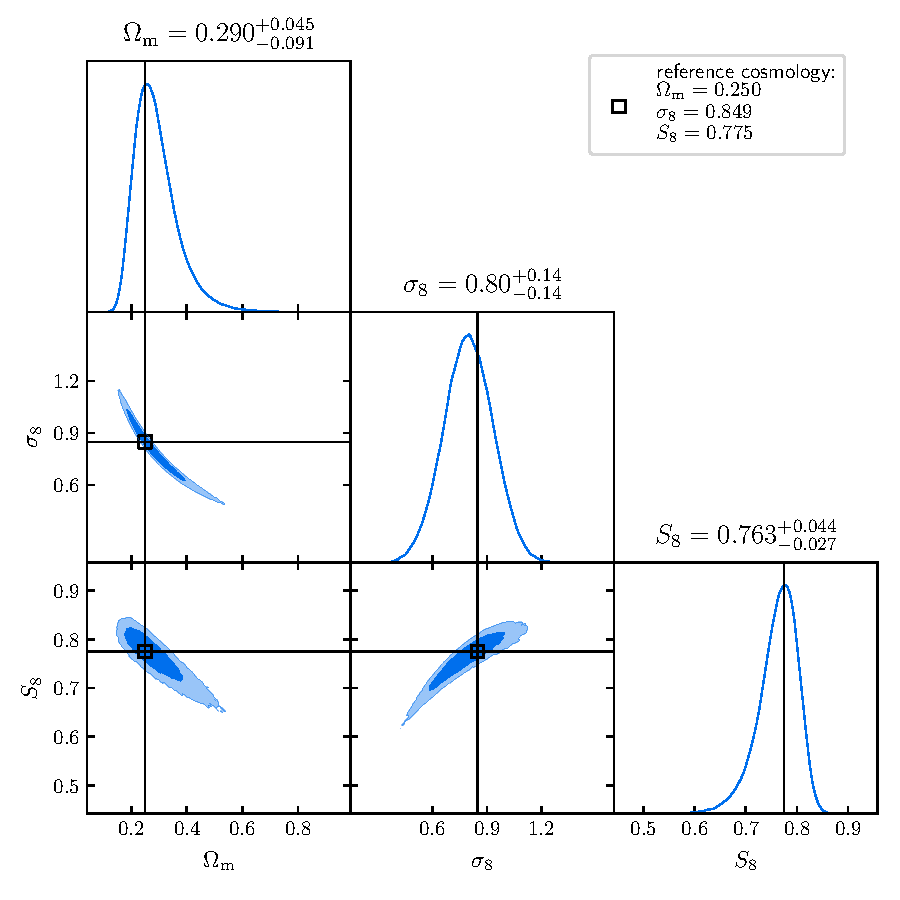
\includegraphics[width=0.7\textwidth]{images/obscorr.pdf}
	\caption{Bias in the parameters for a KiDS-like Survey.}
	\label{fig:mcmc_kids}
\end{figure}  
\begin{figure}[h]
\centering
	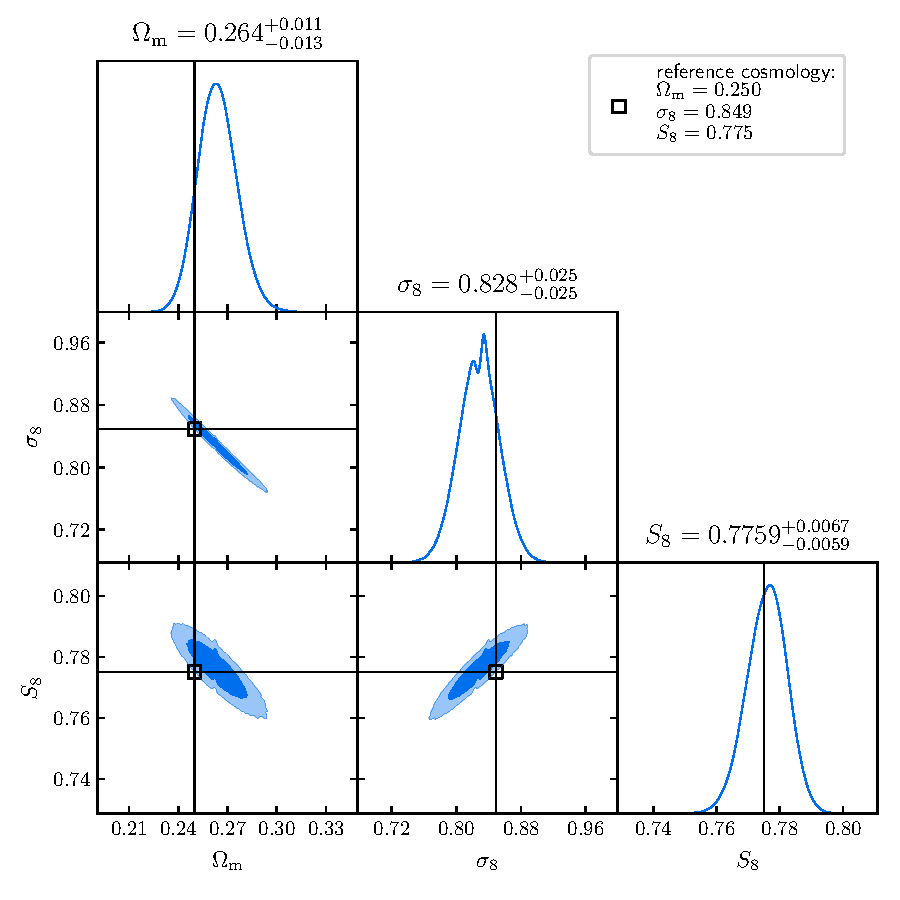
\includegraphics[width=0.7\textwidth]{images/euclid.pdf}
	\caption{Bias in the parameters for a Euclid-like Survey.}
	\label{fig:mcmc_euclid}
\end{figure}  
\todo{Put both in one plot? Maybe put reference MC simulation where $\xi_\pm$ was not changed?}
